\section{Phylogenetics and phylodynamics}
\label{sec:phylo}

\subsection{Phylogenetic trees}

In evolutionary biology, a \defn{phylogeny}, or \defn{phylogenetic tree}, is a
graphical representation of the the evolutionary relationships among a group of
organisms or species (generally, \defn{taxa})~\autocite{haeckel1866generelle}.
The \defn{tips} of a phylogeny, that is, the nodes without any descendants,
correspond to \defn{extant}, or observed, taxa. The \defn{internal nodes}
correspond to their (usually extinct) common ancestors. The edges or
\defn{branches} of the phylogeny connect ancestors to their descendants.
Phylogenies may have a \defn{root}, which is a node with no descendants
distinguished as the most recent common ancestor of all the extant
taxa~\autocite{harding1971probabilities}. When such a root exists, the tree is
referred to as being \defn{rooted}; otherwise, it is \defn{unrooted}. The
structural arrangement of nodes and edges in the tree is referred to as its
\defn{topology}~\autocite{cavalli1967phylogenetic}. 

The branches of the tree may have associated lengths, representing either
evolutionary distance or calendar time between ancestors and their descendants.
The term ``evolutionary distance'' is used here imprecisely to mean any sort of
quantitative measure of evolution, such as the number of differences between
the DNA sequences of an ancestor and its descendant, or the difference in
average body mass or height. A phylogeny with branch lengths in calendar time
units is often referred to as \defn{time-scaled}. In a time-scaled phylogeny,
the internal nodes can be mapped onto a timeline by using the tips of the tree,
which usually correspond to the present day, reference
points~\autocite{nee1992tempo}. The corresponding points on the timeline are
called \defn{branching times}, and the rate of their accumulation is referred
to as the \defn{branching rate}. Rooted trees whose tips are all the same
distance from the root are called \defn{ultrametric}
trees~\autocite{buneman1974note}. These concepts are illustrated in
\cref{fig:speciestree}.

\begin{figure}[ht]
  \centering
  \includegraphics{speciestree.pdf}
  \caption[Illustration of a rooted, ultrametric, time-scaled phylogeny.]
    {Illustration of a rooted, ultrametric, time-scaled phylogeny. The tips of
      the tree, which represent extant taxa, are placed at the present day on
      the time axis. Internal nodes, representing extinct common ancestors to
      the extant taxa, fall in the past. The topology of the tree indicates
      that cats and dogs are the most closely related pair of species, whereas
      fish is most distantly related to any other node in the tree.}
  \label{fig:speciestree}
\end{figure}

\subsection{Transmission trees}

In epidemiology, a \defn{transmission tree} is a graphical representation of an
epidemic's progress through a population~\autocite{ypma2013relating}. Like
phylogenies, transmission trees have tips, nodes, edges, and branch lengths.
However, rather than recording an evolutionary process (speciation), they
record an epidemiological process (transmission). The tips of a transmission
tree represent the removal by sampling of infected hosts, while internal nodes
correspond to transmissions from one host to another. Transmission trees
generally have branch lengths in units of calendar time, with branching times
indicating times of transmission. The root of a transmission tree corresponds
to the initially infected patient who introduced the epidemic into the network,
also known as the \defn{index case}. The internal nodes may be labelled with
the donor of the transmission pair, if this is known. The tips of the tree,
rather than being fixed at the present day, are placed at the time at which the
individual was removed from the epidemic, such as by death, recovery,
isolation, behaviour change, or migration~\autocite{stadler2013uncovering}.
Consequently, the transmission tree may not be ultrametric, but may have tips
located at varying distances from the root. Such trees are said to have
\defn{heterochronous} taxa~\autocite{drummond2003measurably}, in contrast to
the \defn{isochronous} taxa found in most phylogenies of macro-organisms. A
transmission tree is illustrated in \cref{fig:contactnet} (right). 
{\color{blue} The object on the right of the figure is called a \defn{contact
network}, which depicts the entire susceptible population along with all
possible routes of disease transmission. Contact networks, and their
relationships to transmission trees, will be discussed further in
\cref{sec:contactnet}}.

Each infected individual in an epidemic may appear at nodes of the transmission
tree more than once. This is different from the transmission \emph{network}, in
which each infected individual appears exactly once, and edges are in
one-to-one correspondence with transmissions~\autocite{welch2011statistical,
keeling2005networks}. The distinction between the two objects is illustrated in
\cref{fig:contactnet}. However, since transmission networks generally have no
cycles (unless re-infection occurs), they are trees in the graph theoretical
sense, and hence are sometimes also referred to as transmission
trees~\autocite[\eg][]{kenah2015algorithms}. In this work, we reserve the term
``transmission tree'' for the objects depicted on the right side of
\cref{fig:contactnet}, following \eg~\autocite{stadler2013uncovering}. The term
``transmission network'' is taken to mean the subgraph of the contact network
along which transmissions occurred, following
\eg~\autocite{welch2011statistical, keeling2005networks}.

\begin{figure}
    \centering
    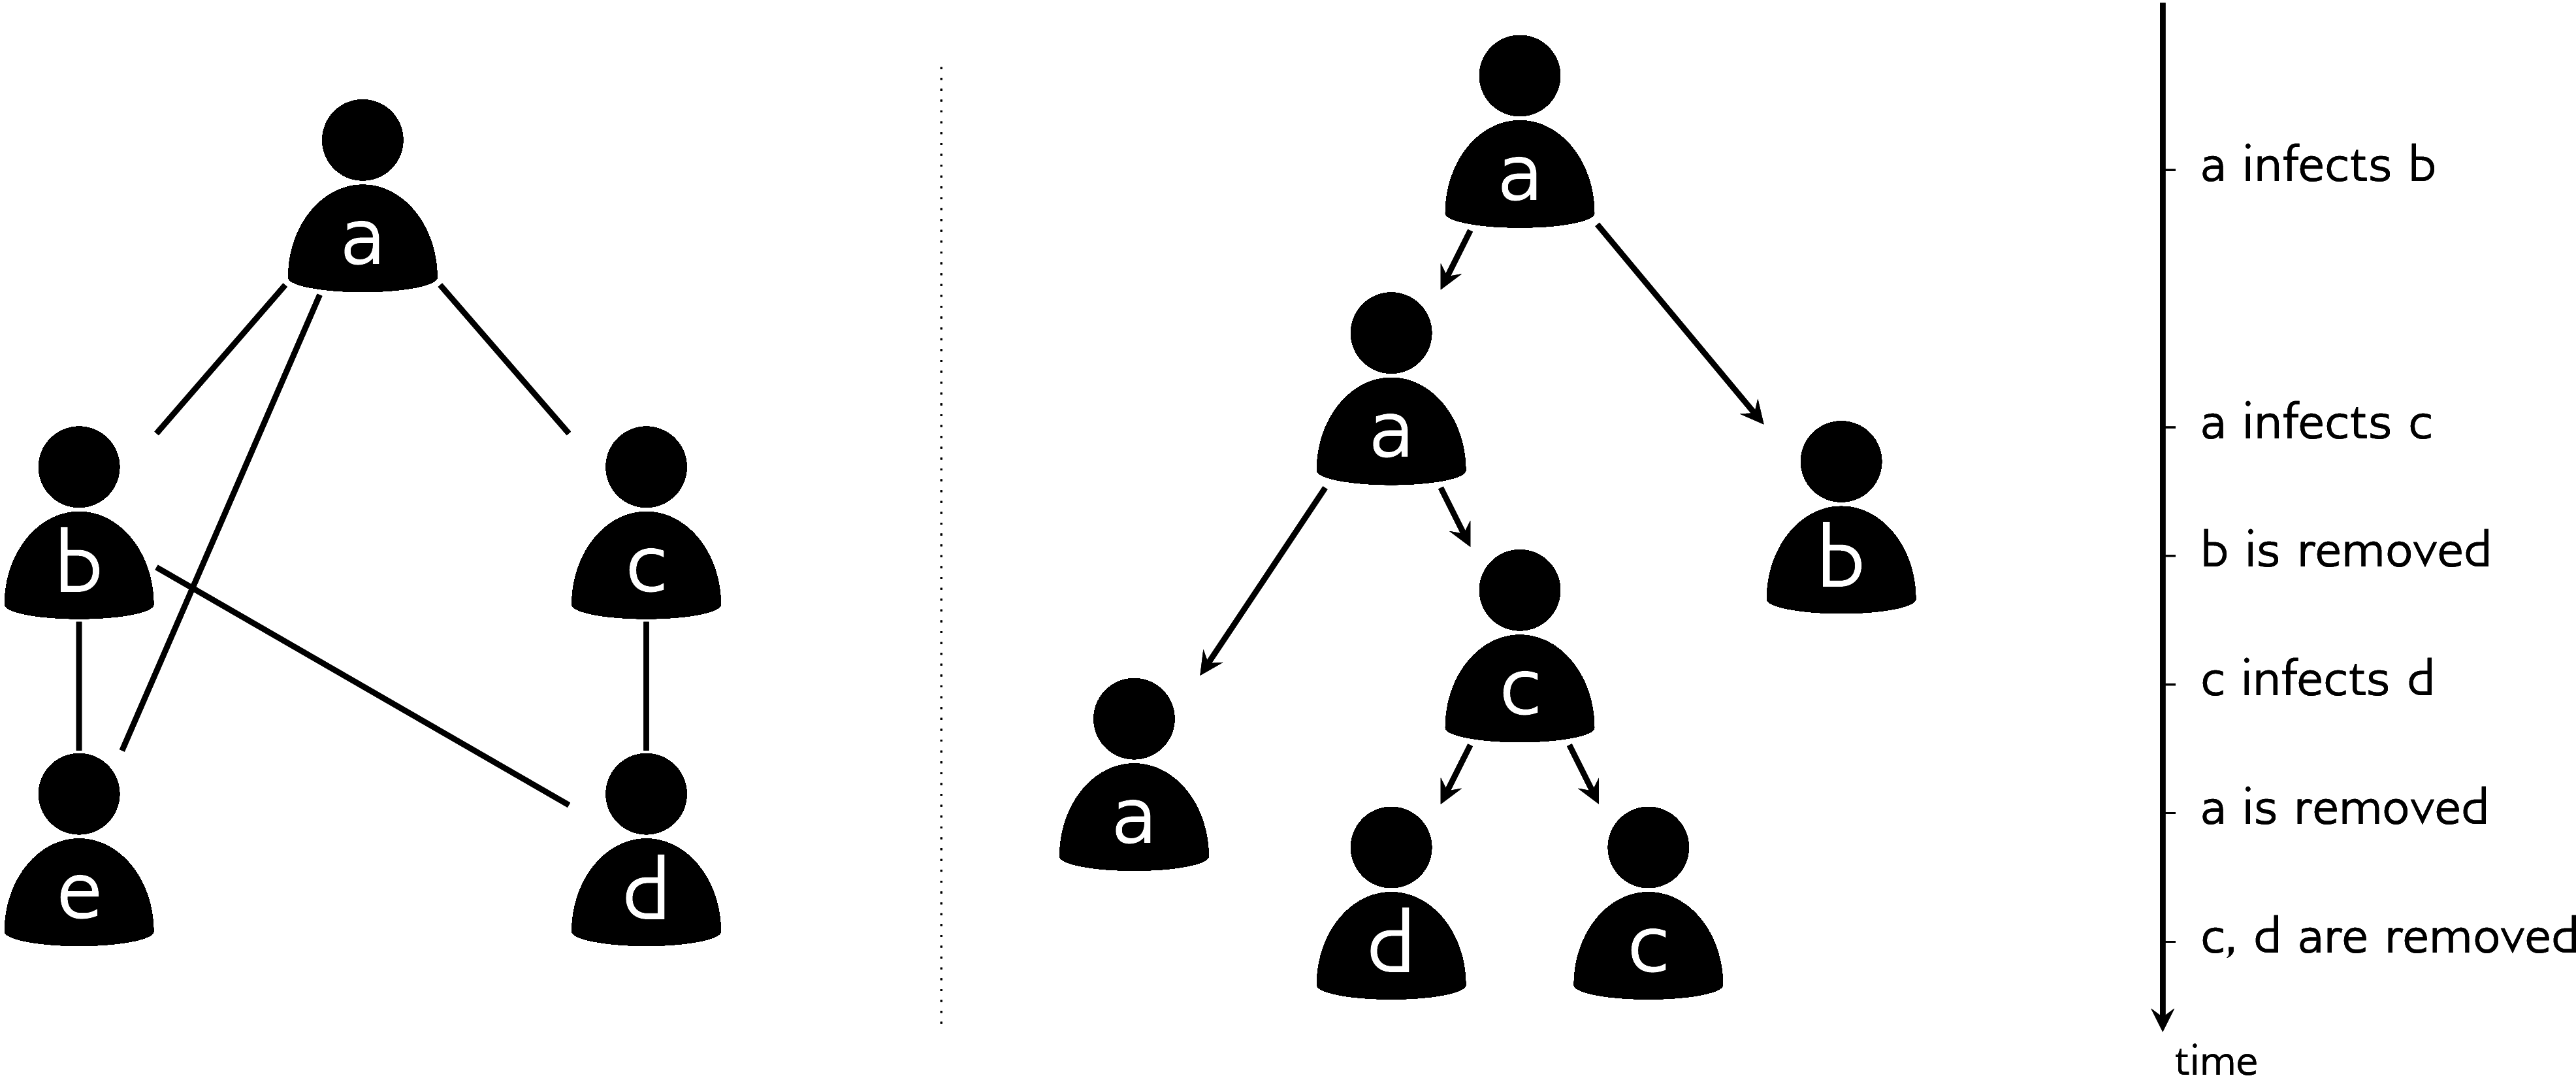
\includegraphics[width=\textwidth]{contactnet.pdf}
    \caption[Illustration of a contact network and transmission tree.]{
      Illustration of epidemic spread over a contact network, and the
      corresponding transmission tree. (Left) A contact network with five
      hosts, labelled $a$ through $e$. Thick shaded edges indicate symmetric
      contacts among the hosts. The transmission network is indicated by
      coloured arrows. The epidemic began with node $a$, who transmitted to
      nodes $b$ and $c$. Node $c$ further transmitted to node $d$. Node $e$ was
      not infected. (Right) The transmission tree corresponding to this
      scenario, with a timeline of transmission and removal times.
    }
    \label{fig:contactnet}
\end{figure}

Since transmission trees are essentially a detailed record of an epidemic's
progress, they contain substantial epidemiological information. As a basic
example, the \gls{ltt} plot~\autocite{nee1992tempo}, which plots the number of
lineages in a phylogeny against time, can be used to quantify the incidence of
new infections over the course of an epidemic~\autocite{holmes1995revealing}.
However, in all but the most well-studied of epidemics, transmission trees are
not possible to assemble through traditional epidemiological
methods~\autocite{welch2011statistical}. The time and effort to conduct
detailed interviews and contact tracing of a sufficient number of infected
individuals is usually prohibitive, and may be additionally be confounded by
misreporting and other challenges~\autocite{eames2015six}. However, it turns
out that for viral epidemics, some of the epidemiological information contained
in the transmission tree leaves a mark on the viral genetic material
circulating in the population. A family of methods called
\defn{phylodynamics}~\autocite{grenfell2004unifying} addresses the challenge of
estimating epidemiological parameters from viral sequence
data~\autocite{volz2013viral}.

\subsection{Phylodynamics: linking evolution and epidemiology}
\label{subsec:phylodynamics}

%Most modern analyses use model-based methods, which simultaneously
%estimate the phylogeny with branch lengths and the parameters of a model of
%evolution. Although they usually work well in practice, the estimated topology
%can vary based on the model used and, in the case of Bayesian analysis, the
%priors. In addition, intra-host viral populations are genetically
%heterogeneous, so choosing a single representative genotype per host is
%necessarily imprecise. One can use either the genotype of a specific virion
%sampled from the host, or a synthetic genotype, such as a consensus or
%reconstructed ancestral sequence.

The basis of phylodynamics is the fact that, for RNA viruses, epidemiological
and evolutionary processes occur on similar time
scales~\autocite{drummond2003measurably}. In fact, these two processes
interact, such that it is possible to detect the influence of host epidemiology
on the evolutionary history of the virus as recorded in an \defn{inter-host
viral phylogeny}. Phylodynamic methods aim to detect and quantify the
signatures of epidemiological processes in these
phylogenies~\autocite{pybus2009evolutionary, volz2013viral}, which relate one
representative viral genotype from each host in an infected population. These
methods have been used to investigate parameters such as transmission rate,
recovery rate, and basic reproductive number~\autocite{pybus2009evolutionary,
volz2013viral}. The majority of phylodynamic studies attempt to infer the
parameters of an epidemiological model for which the likelihood of an observed
phylogeny can be calculated. Most often, this is some variation of the
birth-death~\autocite{kendall1948generalized, stadler2012estimating} or
coalescent~\autocite{kingman1982coalescent, volz2012complex} models. These
methods either assume the viral phylogeny is known, as we do in this work, or
(more commonly) integrate over phylogenetic uncertainty in a Bayesian
framework. Phylogenetic inference is a complex topic which we shall not discuss
here; see \eg~\autocite{nei2000molecular} for a full review.

Due to the relationship between the aforementioned processes, there is a degree
of correspondence between viral phylogenies and transmission
trees~\autocite{leitner2002molecular, ypma2013relating, kenah2015algorithms,
kenah2016molecular}. In particular, the transmission process is quite similar
to \defn{allopatric speciation}~\autocite{coyne2004speciation}, where genetic
divergence follows the geographic isolation of a sub-population of organisms.
Thus, transmission, which is represented as branching in the transmission tree,
causes branching in the viral phylogeny as
well~\autocite{volz2009phylodynamics}. Similarly, the removal of an individual
from the transmission tree causes the extinction of their viral lineage in the
phylogeny. Consequently, the topology of the viral phylogeny is sometimes used
as a proxy for the topology of the transmission
tree~\autocite{hall2015epidemic}. Modern likelihood-based methods of
phylogenetic reconstruction~\autocite[\eg][]{price2010fasttree,
stamatakis2014raxml} produce unrooted trees whose branch lengths measure
genetic distance in units of expected substitutions per site. On the other
hand, transmission trees are rooted, and have branches measuring calendar
time~\autocite{pybus2009evolutionary}. Therefore, estimating a transmission
tree from a viral phylogeny requires the phylogeny to be rooted and
time-scaled. Methods for performing this process include root-to-tip
regression~\autocite{shankarappa1999consistent, korber2000timing,
drummond2003inference}, which we apply in this work, and least-square
dating~\autocite{to2015fast}. Alternatively, the tree may be rooted separately
with an outgroup~\autocite{li1988rates} before time-scaling.

A caveat of estimating transmission trees in this manner is that the
correspondence between the topologies of the viral phylogeny and transmission
tree is far from exact~\autocite{ypma2013relating, romero2014timing}.  Due to
intra-host diversity, the viral strain which is transmitted may have split from
another lineage within the donor long before the transmission event occurred.
Hence, the branching point in the viral phylogeny may be much earlier than that
in the transmission tree. Another possibility is that one host transmitted to
two or more recipients in one order, but the transmitted lineages originated
within the donor in a different order. In this case, the topology of the
transmission tree and the viral phylogeny will be mismatched. In practice, this
discordance has not proven an insurmountable problem: for example,
\textcite{leitner1996accurate, paraskevis2004phylogenetic} were able to
accurately recover a known transmission tree using a viral phylogeny. The
problem of accurately estimating transmission trees is an ongoing area of
research~\autocite{cottam2008integrating, jombart2011reconstructing,
ypma2012unravelling, morelli2012bayesian, didelot2014bayesian}.

%Although phylodynamics is quite new, these phenomena have been studied in
%evolutionary biology for some time. Viral phylogenies are a specific version of
%a more general class of trees called \defn{gene trees}, which represent the
%evolutionary history of a section of genetic material. Transmission trees, on
%the other hand, are highly analogous to \defn{species trees}, whose tips are
%species and internal nodes are common ancestors. This analogy derives from the
%functional similarity between transmission and allopatric speciation. Hence,
%the potential discordance between transmission trees and viral phylogenies is
%the similar to that between gene and species trees, which is called
%\defn{incomplete lineage sorting}. 

%What we have just discussed is a two-step procedure for estimating the
%transmission tree. First, a viral phylogeny is constructed from genetic
%sequence data, and then it is rooted and time-scaled into a transmission tree.
%This approach is straightforward, frequently used, and has the advantage of
%leveraging tried-and-true tools for phylogenetic inference. However, it also
%has drawbacks, perhaps the most obvious being the multiplication of errors
%produced by the separate steps. One commonly used alternative method is to
%directly estimate a time-scaled phylogeny by simultaneously inferring the tree
%topology, its root and branch lengths, and the parameters of a \defn{molecular
%clock} model. A molecular clock is a hypothesis about the evolutionary rates
%along the branches of the tree, such as that they are all equal (a \defn{strict
%clock}) or that they are \gls{iid} from a common distribution (a \defn{relaxed
%clock}). This inference is usually done in a Bayesian framework using
%\gls{MCMC}, so that prior information (including the tip dates) can be included
%in the analysis, and the so-called nuisance parameters of the molecular clock
%model can be marginalized out. Software packages for performing these analyses
%include BEAST~\autocite{bouckaert2014beast} and
%MrBayes~\autocite{ronquist2012mrbayes}.

%Other methods are tailor-made for inferring transmission trees.
%\textcite{didelot2014bayesian} develop a Bayesian approach which allows
%transmissions to occur anywhere along the
%branches of a transmission tree, rather than being constrained to the branching
%points in the viral phylogeny. The method requires sampling of every infected
%individual, although the authors indicate that it could be extended to relax
%this assumption. \textcite{cottam2008integrating} describe a likelihood-based
%method which enumerates all transmission trees consistent with an established
%phylogeny, assigning each a likelihood based on other epidemiological data.
%This approach is novel in its integration of data from multiple sources,
%however because it enumerates a large portion of the tree space, it is unlikely
%to scale to larger epidemics. \textcite{ypma2012unravelling} develop a joint
%likelihood function integrating temporal, geographic, and genetic observations,
%and use Bayesian \gls{MCMC} to estimate both the tree and the parameters of the
%likelihood function. Their approach can handle missing data and produces high
%resolution transmission trees when multiple types of data are available. A
%different approach is undertaken by \textcite{jombart2011reconstructing}, who
%describe a method to build transmission trees directly from sequence data,
%contingent on the common ancestors also being sampled. This makes the method
%attractive for slow-evolving pathogens, but less practical for viral outbreaks
%where samples from common ancestors are unlikely to be available.

\subsection{Tree shapes}
\label{subsec:treeshape}

To perform phylodynamic inference, we must be able to extract quantitative
information from viral phylogenies. What is informative about a phylogeny,
beyond the demographic characteristics of the individuals it relates, is its
\defn{shape}. The shape of a phylogeny has two components: the topology, and
the distribution of branch lengths~\autocite{mooers1997inferring}. Methods of
quantifying tree shape fall into two categories: summary statistics, and
pairwise measures. Summary statistics assign a numeric value to each individual
tree, while pairwise measures quantify the similarity between pairs of trees. 

One of the most widely used tree summary statistics is Sackin's
index~\autocite{shao1990tree}, which measures the imbalance or asymmetry in a
rooted tree. For the $i$th tip of the tree, we define $N_i$ to be the number of
branches between that tip and the root. The unnormalized Sackin's index is
defined as the sum of all $N_i$. It is called unnormalized because it does not
account for the number of tips in the tree. Among two trees having the same
number of tips, the least-balanced tree will have the highest Sackin's index.
However, among two equally balanced trees, the larger tree will have a higher
Sackin's index. This makes it challenging to compare balances among trees of
different sizes. To correct this, \textcite{kirkpatrick1993searching} derive
the expected value of Sackin' index under the Yule
model~\autocite{yule1925mathematical}. Dividing by this expected value
normalizes Sackin's index, so that it can be used to compare trees of different
sizes. An example of a pairwise measure is the
\gls{nltt}~\autocite{janzen2015approximate}, which compares the
\gls{ltt}~\autocite{nee1992tempo} plots of two trees. Specifically, the two
\gls{ltt} plots are normalized so that they begin at $(0, 0)$ and end at $(1,
1)$, and the absolute difference between the two plots is integrated between 0
and 1. In the context of infectious diseases, the \gls{ltt} is related to the
prevalence~\autocite{holmes1995revealing}, so large values may indicate that
the trees being compared were produced by different epidemic
trajectories~\autocite{janzen2015approximate}.

\textcite{poon2013mapping} developed an alternative pairwise measure which
applies the concept of a \defn{kernel function} to phylogenies. Kernel
functions, originally developed for \glspl{SVM}~\autocite{burges1998tutorial}, 
compare objects in a space $\X$ by mapping them into a feature space $\F$ of
high or infinite dimension via a function $\varphi$. The similarity between the
objects is defined as
\[  
  K(x, x') = \langle \varphi(x), \varphi(x')\rangle,
\]
that is, the inner product of the objects' representations in the feature
space. Computing $\varphi(x)$ may be computationally prohibitive due to the
dimension of $\F$. The utility of a kernel function $K$ is that it is
constructed in such a way that it can compute the inner product without
explicitly computing $\varphi(x)$. The kernel function developed in
\autocite{poon2013mapping} will henceforth be referred to as the \defn{tree
kernel}. This kernel maps trees into the space of all possible possible
\defn{subset trees}, which are subtrees that do not necessarily extend all the
way to the tips. The subset-tree kernel was originally developed for comparing
parse trees in natural language processing~\autocite{collins2002new} and did
not incorporate branch length information. The version developed by
\textcite{poon2013mapping} includes a radial basis function to compare the
differences in branch lengths, thus incorporating both the trees' topologies
and their branch lengths in a single similarity score. 

The kernel score of a pair of trees, denoted $K(T_1, T_2)$, is defined as a sum
over all pairs of nodes $(n_1, n_2)$, where $n_1$ is a node in $T_1$ and $n_2$
is a node in $T_2$. Following \textcite{poon2013mapping}, let $N(T)$ denote the
set of all nodes in $T$, $\nc(n)$ be the number of children of node $n$,
$c_n^{j}$ be the $j$th child of node $n$, and $l_n$ be the vector of branch
lengths connecting node $n$ to its descendants. The \defn{production rule} of
$n$ is its total number of children, and its number of leaf children. That is,
if two nodes have the same number of children and among these, the same number
of leaves, then they have the same production rule. Let $k_G(x, y)$ be a
Gaussian radial basis function of the vectors $x$ and $y$,
\[
  k_G(x, y) = \exp\left(-\frac{1}{2\sigma} \norm{x - y}_2^2\right),
\]
where $\norm{\cdot}_2$ is the Euclidean norm and $\sigma$ is a variance
parameter. The tree kernel is defined as 
\[
  K(T_1, T_2) = \sum_{n_1 \in N(T_1)} \sum{n_2 \in N(T_2)} \Delta (n_1, n_2),
\]
where
\[
  \Delta(n_1, n_2) =
  \begin{cases}
    \lambda & n_1 \text{ and } n_2 \text{ are leaves} \\
    \lambda k_G(l_{n_1}, l_{n_2}) \displaystyle\prod_{j=1}^{\nc(n_1)} \left(1 +
    \Delta(c_{n_1}^j, c_{n_2}^j) \right) & \begin{aligned} n_1 \text{ and } n_2 \text{ have the same} \\ \text{production rule} \end{aligned} \\
    0 & \text{otherwise}.

  \end{cases}
\]
Here $\lambda$ is a decay factor parameter, which penalizes large matches that
tend to dominate the kernel score. In this work, we refer to the parameters
$\lambda$ and $\sigma$ as \defn{meta-parameters}, to avoid confusing them with
model parameters we are trying to estimate.

%The tree kernel was later shown to be highly effective in differentiating trees
%simulated under a compartmental model with two risk groups of varying contact
%rates~\autocite{poon2015phylodynamic}. In that paper,
%\citeauthor{poon2015phylodynamic} used the tree kernel as the distance function
%in \gls{ABC} (see \cref{sec:abc}), to fit epidemiological models to observed
%trees. This is an example of kernel-ABC~\autocite{nakagome2013kernel}, which
%will be discussed further in \cref{sec:abc}.

\section{Contact networks}
\label{sec:contactnet}

\subsection{Overview}
\label{subsec:netoverview}

Epidemics spread through populations of hosts through \defn{contacts} between
those hosts. The definition of contact depends on the mode of transmission of
the pathogen in question. For an airborne pathogen like influenza, a contact
may be simple physical proximity, while for \gls{HIV}, contact could be via
unprotected sexual relations or blood-to-blood contact (such as through needle
sharing). A \defn{contact network} is a graphical representation of a host
population and the contacts among its members~\autocite{klovdahl1985social,
morris1993epidemiology, keeling2005networks}. The \defn{nodes} in the network
represent hosts, and \defn{edges} or \defn{links} represent contacts between
them. A contact network is shown in \cref{fig:contactnet} (left). Contact
networks are a particular type of \defn{social
network}~\autocite{moreno1953shall, barnes1954class}, which is a network in
which edges may represent any kind of social or economic relationship. Social
networks are frequently used in the social sciences to study phenomena where
relationships between people or entities are important \autocite[for a review
see][]{wasserman1994social}.

Edges in a contact networks may be \defn{directed}, representing one-way
transmission risk, or \defn{undirected}, representing symmetric transmission
risk. For example, a network for an airborne epidemic would use undirected
edges, because the same physical proximity is required for a host to infect or
to become infected. However, an infection which may be spread through
blood-to-blood contact through transfusions transfusions would use directed
edges, since the donor has no chance of transmitting to the recipient. Directed
edges are also useful when the transmission risk is not equal between the
hosts, such as with \gls{HIV} transmission among \gls{MSM}, where the receptive
partner carries a higher risk of infection than the insertive
partner~\autocite{baggaley2010hiv}. In this case, a contact could be
represented by two directed edges, one in each direction between the two hosts,
with the edges annotated by what kind of risk they
imply~\autocite{wasserman1994social}. An undirected contact network is
equivalent to a directed network where each contact is represented by two
symmetric directed edges. The \defn{degree} of a node in the network is how
many contacts it has. In directed networks, we may make the distinction between
\defn{out-degree} and \defn{in-degree}, which count respectively the number
incoming and outgoing edges. The \defn{degree distribution} of a network
denotes the probability that a node has any given number of links. The set of
edges attached to a node are referred to as its \defn{incident} edges.

Epidemiological models most often assume some form of contact homogeneity. The
simplest models, such as the \gls{SIR} model~\autocite{anderson1992infectious},
assume a completely homogeneously mixed population, where every pair of
contacts is equally likely. More sophisticated models partition the population
into groups with different contact rates between and among each
group~\autocite{jacquez1988modeling}. However, these models still assume that
every possible contact between a member of group $i$ and a member of group $j$
is equally likely. This assumption is clearly unrealistic for the majority of
human communities, and can lead to errors in predicted epidemic trajectories
when there is substantial heterogeneity present~\autocite{bansal2007individual,
volz2007susceptible, rolls2015simulation}. Contact networks provide a way to
relax this assumption by representing individuals and their contacts
explicitly. It is important to note that, although panmixia is an unrealistic
modelling assumption, it has not proven a substantial hurdle to epidemic
modelling in practice~\autocite{anderson1992infectious}. Using this assumption,
researchers have been able to derive estimates of the transmission rate and the
basic reproductive number of various outbreaks, which have agreed with values
obtained by on-the-ground data collection~\autocite{stadler2014insights}.
Therefore, if one is interested only in these population-level variables, the
additional complexity of contact network models may not be warranted. Rather,
these models are most useful when we are interested in properties of the
network itself, such as centrality, structural balance, and
transitivity~\autocite{wasserman1994social}.

From a public health perspective, knowledge of contact networks has the
potential to be extremely useful. On a population level, network structure can
dramatically affect the speed and pattern of epidemic
spread~\autocite[\eg][]{barthelemy2005dynamical, volz2008sir}. For example,
epidemics are expected to spread more rapidly in networks having the ``small
world'' property, where the average path length between two nodes in the
network is relatively low~\autocite{watts1998collective}. Some sexually
transmitted infections would not be expected to survive in a homogeneously
mixed population, but their long-term persistence can be explained by contact
heterogeneity~\autocite{anderson1992infectious, pastor2001epidemic}. Hence, the
contact network can provide an idea of what to expect as an epidemic unfolds.
In terms of actionable information, the efficacy of different vaccination
strategies may depend on the topology of the
network~\autocite{keeling2005networks,peng2013vaccination, ma2013importance,
rushmore2014network}. On a local level, contact networks can be informative
about the groups or individuals who are at highest risk of acquiring or
transmitting infection, and would therefore benefit most from public health
interventions~\autocite{wang2015targeting, little2014using}.

Contact networks are a challenging type of data to collect, requiring extensive
epidemiological investigation in the form of contact
tracing~\autocite{morris1993epidemiology, welch2011statistical,
keeling2005networks, eames2015six}. Therefore, it has been necessary to explore
less resource-intensive alternatives which still contain information about
population structure. For instance, it is possible to obtain limited
information about the contact network by individual interviews without contact
tracing. Variables which can be estimated in this fashion are referred to as
\defn{node-level} measures~\autocite{wasserman1994social}. One of the most
well-studied of these is the degree distribution mentioned above, which can
theoretically be estimated by simply asking each person how many contacts they
had in some interval of time. However, the degree distributions often observed
in real-world sexual networks are heavy-tailed~\autocite{liljeros2001web,
schneeberger2004scale, colgate1989risk}, so dense or respondent-driven
sampling~\autocite{heckathorn1997respondent} would be needed to capture the
high-degree nodes characterizing the tail of the distribution.

An alternative approach has been the analysis of other types of network, which
can be directly estimated with phylogenetic methods from viral sequence data.
Some work focuses on the \defn{phylogenetic network}, in which two nodes are
connected if the genetic distance between their viral sequences is below some
threshold.  Primarily, this work has focused on the detection of
\defn{phylogenetic clusters}, which are groups of individuals whose viral
sequences are significantly more similar to each other's than to the general
population's.  The phylogenetic network is informative about ``hotspots'' of
transmission and can be used to identify demographic groups to whom targeted
interventions are likely to have the greatest effect~\autocite{poon2015impact}.
However, this network may show little to no agreement with a contact data
obtained through epidemiological methods~\autocite{yirrell1998molecular,
resik2007limitations, robinson2013dynamics}, and therefore may be a poor proxy
for the contact network. Other studies~\autocite{brown2011transmission} have
investigated the \defn{transmission network}, which is the subgraph of the
contact network consisting of infected nodes and the edges which led to their
infections~\autocite{welch2011statistical} (\cref{fig:contactnet}, left). It is
possible to estimate the transmission network phylogenetically, although the
methods required for doing so are more sophisticated than for estimating the
phylogenetic network~\autocite{brown2011transmission}. These studies again
mostly focusing on clustering, and also on degree distributions.

Other statistical methods have been developed to infer contact network
parameters strictly from the timeline of an epidemic, using neither genetic
data nor reported contacts. \textcite{britton2002bayesian} developed a Bayesian
method to infer the $p$ parameter of an \gls{ER} network, along with the
transmission and removal rate parameters of the \gls{SI} model, using observed
infection and optionally removal times. However, it was designed for only a
small number of observations, and was unable to estimate $p$ independently from
the transmission rate.  \textcite{groendyke2011bayesian} significantly updated
and extended the methodology of \citeauthor{britton2002bayesian}, and applied
it to a measles outbreak affecting 188 individuals. They were able to obtain a
much more informative estimate of $p$, although this data set included both
symptom onset and recovery times for all individuals, and was unusual in that
the entire contact network was presumed to be infected. \textcite{volz2008sir}
developed differential equations describing the dynamics of the \gls{SIR} model
on a wide variety of random networks defined by their degree distributions.
Although the topic of estimation was not addressed in the original paper,
\citeauthor{volz2008sir}'s method could in principle be used to fit such models
to observed epidemic trajectories, similar to what is done with the ordinary
\gls{SIR} model. \textcite{volz2007susceptible} later extended the method to
dynamic contact networks and applied it to a sexual network relating 99
individuals investigated during a syphilis outbreak.

\subsection{Scale-free networks and preferential attachment}
\label{subsec:pa}

A \defn{scale-free} network is one whose degree distribution follows a power
law, meaning that the number of nodes in the network with degree $k$ is
proportional to $k^{-\gamma}$ for some constant
$\gamma$~\autocite{barabasi1999emergence}. Scale-free networks are
characterized by a large number of nodes of low degree, with relatively few
``hub'' nodes of very high degree. Epidemiological surveys have indicated that
human sexual networks tend to be scale-free~\autocite{liljeros2001web,
schneeberger2004scale, colgate1989risk, clemenccon2015statistical}.
Interestingly, many other types of network, including computer
networks~\autocite{pastor2001epidemic}, biological metabolic
networks~\autocite{jeong2000large}, and academic co-author
networks~\autocite{barabasi2002evolution}, also have the scale-free property.

Several properties of scale-free networks are relevant in epidemiology.  The
high-degree hub nodes are known as
\defn{superspreaders}~\autocite{kemper1980identification}, which have been
postulated to contribute in varying degree to the spread of diseases such as
\gls{HIV}~\autocite{stadler2013uncovering} and
\gls{SARS}~\autocite{shen2004superspreading}. Scale-free networks have no
epidemic threshold~\autocite{pastor2001epidemic}, meaning that diseases with
arbitrarily low transmissibility can persist at low levels indefinitely. This
is in contrast with homogeneously mixed populations, in which transmissibility
below the epidemic threshold would result in exponential decay in the number of
infected individuals and eventual extinction of the
pathogen~\autocite{anderson1992infectious}.

One mechanism which has been shown to lead to scale-free networks is
\defn{preferential attachment}~\autocite{simon1955class,
barabasi1999emergence}. The simplest preferential attachment model is known as
the \gls{BA} model after its inventors~\autocite{barabasi1999emergence}. Under
this model, networks are formed by starting with a small number $m_0$ of nodes.
New nodes are added one at a time until there are a total of $N$ in the
network. Each time a new node is added, $m \geq 1$ edges are added from it to
other nodes in the graph. In the original formulation, the partners of the new
node are chosen with probability linearly proportional to their degree.
However, \citeauthor{barabasi1999emergence} suggest extending the model such
that the probability of choosing a partner of degree $d$ is proportional to
$d^\alpha + 1$ for some constant $\alpha$, and we use this extension here. When
$m = 1$, the network takes on the distinctive shape of a tree, that is, it does
not contain any cycles. Cycles are present in the network for all all other $m$
values.

There has been some contention of the idea that contact networks are
scale-free. \textcite{handcock2004likelihood} fit several stochastic models of
partner formation to empirical degree distributions derived from population
surveys of sexual behaviour. They found that a negative binomial distribution,
rather than a power law, was the best fit to five out of six datasets, although
the difference in goodness of fit was extremely small in four out of these
five. \textcite{bansal2007individual} found that an exponential distribution,
rather than a power law, was the best fit to degree distributions of six social
and sexual networks. 

\subsection{Relationship between network structure and transmission trees}

The contact network underlying an epidemic constrains the shape of the
transmission network, which in turn determines the topology of the transmission
tree relating the infected hosts (\cref{fig:contactnet}). The index case who
introduces the epidemic into the network becomes the root of the tree. Each
time a transmission occurs, the lineage corresponding to the donor host in the
tree splits into two, representing the recipient lineage and the continuation
of the donor lineage. \Cref{fig:contactnet} illustrates this correspondence.
It must be emphasized that, although the order and timing of transmissions
determines the tree topology uniquely, the converse does not hold. That is, for
any given topology, there are in general many transmission networks which would
lead to that topology. In other words, it impossible to distinguish who
transmitted to whom from a transmission tree alone~\autocite{bernard2007hiv}.

A number of studies have made progress in quantifying the relationship between
contact networks and transmission trees. \textcite{o2011contact} simulated
epidemics over networks with four types of degree distribution. They then
estimated the Bayesian skyride~\autocite{minin2008smooth} population size
trajectory in two ways: from the phylogeny, using \gls{MCMC}; and from the
incidence and prevalence trajectories, using the method developed by
\textcite{volz2009phylodynamics}. The concordance between the two skyrides, as
well as the relationship between the skyride and prevalence curve, was
qualitatively different for each degree distribution.
\textcite{leventhal2012inferring} investigated the relationship between
transmission tree imbalance and several epidemic parameters under four contact
network models, and found that these relationships varied considerably
depending on which model was being considered. The authors also investigated a
real-world \gls{HIV} phylogeny and found a level of unbalancedeness
inconsistent with a randomly mixing population. \textcite{welch2011network}
simulated transmission trees over networks with varying degrees of community
structure. They found that transmission trees simulated under networks with low
clustering could not generally be distinguished from those simulated under
highly clustered networks, and concluded that contact network clusters do not
affect transmission tree shape. However, more recently,
\textcite{villandre2016assessment} investigated the correspondence between
contact network clusters and transmission tree clusters, and did find a
moderate correspondence between the two in some cases.

\section{Sequential Monte Carlo}
\label{sec:smc}

\glsreset{SMC}

\subsection{Overview and notation}

\Gls{SMC} is the name for a family of statistical inference methods which rely
on approximating probability distributions of interest with large collections
of \defn{particles}, here denoted
$\set{x^{(k)}}$~\autocite{doucet2001introduction, liu2008monte}. These
collections or \defn{populations} are constructed to form a \defn{Monte Carlo
approximation} to some distribution of interest $\pi$, meaning that the
empirical distribution of the particles converges in distribution to $\pi$ as
the population size gets large~\autocite{liu2001theoretical}. The word
\defn{sequential} is used because the particle populations are modified in an
iterative fashion over time, for example, to incorporate new evidence. 

To fully describe \gls{SMC}, we will introduce some notation and terminology.
The definitions of these terms will become clearer as they are used. For a
sequence $x_1, \ldots, x_d$, we will write $\vec{x_i}$ to mean the partial
sequence $x_1, \ldots, x_i$. The subscript $^{(k)}$ will be used to indicate
the $k$th particle in a population. To ease the notational burden we will omit
the superscripts and subscripts on the weight functions $w$.

We define a \defn{Markov kernel} as the continuous analogue of the transition
matrix in a finite-state Markov model.  For some spaces $X$ and $Y$, $K \maps X
\times Y \to [0, 1]$ such that
\begin{align}
    \label{eq:mk}
    \int_Y K(x, y) \d y = 1
\end{align}
for all $x \in X$. This is an ``operational'' definition of Markov kernel which
will be suitable for our purposes. A more rigorous definition can be found in
\eg~\autocite{kallenberg2006foundations}. Note that a Markov kernels have
nothing to do with the kernel functions defined in \cref{subsec:treeshape},
other than sharing a name (the word ``kernel'' is ubiquitous in mathematics).

\subsection{Sequential importance sampling}
\label{subsec:sis}

\Gls{SIS}~\autocite{gordon1993novel} is one type of \gls{SMC} method, whose aim
is to sample from a distribution $\pi$ on an high-dimensional space, say
$\pi(\vec{x}) = \pi(x_1, \ldots, x_d)$. The basis of \gls{SIS} is \gls{IS},
which is a method of estimating summary statistics of distributions which are
known only up to a normalizing constant, and therefore cannot be sampled from
directly. That is, if $\pi$ is such a distribution and $f$ is any real-valued
function, \gls{IS} is concerned with estimating
\[
  \pi(f) = \int f(x)\pi(x)\d x = \int f(x) \frac{\gamma(x)}{Z} \d x,
\]
where the integral is over the space on which $\pi$ is defined, $\gamma(x)$ is
known pointwise, and $Z = \int \gamma(x) \d x$ is the unknown normalizing
constant. Suppose we have at hand another distribution $\eta$, called the
\defn{importance distribution}, from which we are able to sample. Define the
\defn{importance weight} as the ratio $w(x) = \gamma(x)/\eta(x)$. We can
express the normalizing constant $Z$ in terms of the importance weight and
distribution, $Z = \int w(x) \eta(x) \d x$, and in turn write the expectation
of interest as
\[
  \int f(x) \pi(x) \d x = \frac{\int f(x) \gamma(x) \d x}
                               {\int w(x) \eta(x) \d x}.
\]
If we sample a large number of points from $\eta$, then $\eta(x)$ can be
approximated by a Monte Carlo estimate. Since the remaining quantities $f$,
$\gamma$, and $w$ can all be evaluated pointwise, these are all the ingredients
we need to obtain an estimate of $\pi(f)$. Although this is a simple and
elegant approach, the drawback is that the variance of the estimate is
proportional to the variance of the importance weights~\autocite{liu2008monte},
which may be quite large if $\eta$ and $\gamma$ are very different. Therefore,
the practical use of \gls{IS} on its own is limited, since it depends on
finding an importance distribution similar to $\pi$, which we usually know very
little about \textit{a priori}.

The objective of \gls{SIS} is to build up an importance distribution $\eta$ for
$\pi$ sequentially. By the general product rule, $\pi(\vec{x})$ can be
decomposed as
\[
  \pi(\vec{x}) 
  = \pi(x_1) \pi(x_2 \mid x_1) \cdots
    \pi(x_{d-1} \mid \vec{x_{d-2}}) \pi(x_d \mid \vec{x_{d-1}}).
\]
This decomposition is natural in many contexts, particularly for on-line
estimation. For example, in a stateful model like an \gls{HMM}, $x_i$ may
represent the state at time $i$, with $\pi(\vec{x})$ being the posterior
distribution over possible paths. The importance distribution $\eta$ for $\pi$
will be constructed using a similar decomposition,
\[
  \eta(\vec{x}) 
  = \eta(x_1) \eta(x_2 \mid x_1) \cdots
    \eta(x_{d-1} \mid \vec{x_{d-2}}) \eta(x_d \mid \vec{x_{d-1}}).
\]
The importance weights for $\eta$ can be written recursively as
\begin{align}
  \label{eq:sisw}
  w(\vec{x_i}) = \frac{\pi(\vec{x_i})}{\eta(\vec{x_i})}
  = \frac{\pi(x_i \mid \vec{x_{i-1}})\pi(\vec{x_{i-1}})}
         {\eta(x_i \mid \vec{x_{i-1}})\eta(\vec{x_{i-1}})}
  = \frac{\pi(x_i \mid \vec{x_{i-1}})}
         {\eta(x_i \mid \vec{x_{i-1}})}\cdot w(\vec{x_{i-1}}).
\end{align}
Thus, we can choose $\eta(x_i \mid \vec{x_{i-1}})$ such that the variance of
the importance weights is as small as possible at every step, eventually
arriving at a full importance distribution. This choice is made on a
problem-specific basis, taking any available information about $\pi(x_i \mid
\vec{x_{i-1}})$ into account (see \textit{e.g.}
\autocite{smith2013sequential,liu2008monte} for many examples).  One potential
choice for $\eta(x_i \mid \vec{x_{i-1}})$ is simply $\pi(x_i \mid
\vec{x_{i-1}})$, if it is possible to compute. In a Bayesian setting, the
prior distribution may be used. The exact form of $\eta(x_i \mid
\vec{x_{i-1}})$ which minimizes the variance of the weights is called the
\defn{optimal kernel}~\autocite{cappe2007overview}, the name deriving from the
fact that $k(x_i, \vec{x_{i-1}}) = \eta(x_i \mid \vec{x_{i-1}})$ is a Markov
kernel. In some applications, it is possible to approximate the optimal kernel
or even compute it explicitly.

The recursive definition \cref{eq:sisw} suggests an algorithm for obtaining a
sample from $\pi$ (\cref{alg:sis}).  We begin with $n$ ``particles'' which have
been sampled from the importance distribution $\eta(x_0)$ for $\pi(x_0)$. The
particles are updated and reweighted $d$ times, corresponding to the $d$
elements of the decomposition of $\pi$. At the $i$th step, each particle is
extended to include $x_i$ drawn according to the chosen $\eta(x_i \mid
\vec{x_{i-1}})$, and the importance weights are recalculated and normalized. 

\begin{algorithm}
  \caption{Sequential importance sampling.}
  \begin{algorithmic}
    \For {$k = 1$ to $n$}
      \State Sample $x_1^{(k)}$ from $\eta(x_1)$
      \Comment{Initialize the $k$th particle}
      \State $w^{(k)} \gets \dfrac{\pi\left(x_1^{(k)}\right)}{\eta\left(x_1^{(k)}\right)}$
    \EndFor
    \For {$i = 2$ to $d$}
      \For {$k = 1$ to $n$}
        \State Sample $x_i^{(k)}$ from $\eta\left(x_i \mid \vec{x_{i-1}^{(k)}}\right)$
        \Comment Extend the $k$th particle
        \State $w(\vec{x_i}^{(k)}) \gets \dfrac{\pi\left(x_i^{(k)} \mid \vec{x_{i-1}^{(k)}}\right)}{\eta\left(x_i^{(k)} \mid \vec{x_{i-1}^{(k)}}\right)} \cdot w(\vec{x_{i-1}}^{(k)})$
      \EndFor
      \State Normalize the weights so that $\sum w = 1$
    \EndFor
    \State Sample $n$ particles with probabilities $w$
  \end{algorithmic}
  \label{alg:sis}
\end{algorithm}

Of course, $\eta$ is merely an approximation to $\pi$, and may be a fairly poor
one depending on the application. Try as we might to keep the variances of the
weights low, the cumulative errors at each sequential step tend to push many of
the weights to very low values. This results in a poor approximation to $\pi$,
since only a few particles retain high importance weights after all $d$
sequential steps. To mitigate this problem, a resampling step is periodically
applied when the variance in the importance weights becomes too high. Several
different criteria have been proposed for when to resample, but we focus here
on the one described by \textcite{liu2008monte}, namely the decay of the
\gls{ESS} below a prescribed threshold, conventionally $n/2$. The \gls{ESS} of
the population of particles is defined as \[ \ESS(w) = \frac{n}{1 + \Var(w)},
\] where $n$ is the number of particles~\autocite{liu2008monte}. When the
\gls{ESS} drops below the threshold, particles are resampled according to their
weights. This results in the removal of low-weight particles from the
population, and also equalizes all the weights. Various resampling strategies
beyond the basic sampling with replacement have been
proposed~\autocite{douc2005comparison}, but we will not discuss those here. 

\subsection{The sequential Monte Carlo sampler}
\label{subsec:smcsamp}

The \gls{SIS} algorithm described above aims to sample from a high-dimensional
distribution $\pi(x)$, by sequentially sampling from $d$ distributions of lower
but increasing dimension. \textcite{del2006sequential} developed an
\defn{\gls{SMC} sampler} with an alternative objective: to sample sequentially
from $d$ distributions $\pi_1, \ldots, \pi_d$, all of the same dimension and
defined on the same space. The $\pi_i$ are assumed to form a related sequence,
such as posterior distributions attained by sequentially considering new
evidence. As with \gls{SIS}, we assume that $\pi_i(x) = \gamma_i(x) / Z_i$,
where $\gamma_i$ is known pointwise and the normalizing constant $Z_i$ is
unknown.

Both algorithms involve progression through a sequence of related
distributions. For \gls{SIS}, these distributions are lower-dimensional
marginals of the target distribution, while for the \gls{SMC} sampler, they are
of the same dimension and constitute a smooth progression from an initial to a
final distribution. In both cases, the neighbouring distributions in the
sequence are related to each other in some way, and we can take advantage of
that relationship to create a sequence of importance distributions alongside
the sequence of targets. In \gls{SIS}, the neighbouring marginals
$\pi(\vec{x_i})$ and $\pi(\vec{x_{i+1}})$ were related by the conditional
density $\pi(x_i \mid \vec{x_{i-1}})$, which we used to inform the importance
distribution. In \gls{SMC}, the relationship between subsequent distributions
is less explicit, but it is assumed that they are related closely enough that
an importance distribution for $\pi_i$ can be easily transformed into one for
$\pi_{i+1}$. In particular, the sequence of importance distributions $\eta_i$
is constructed as
\begin{align}
  \label{eq:impint}
  \eta_i(x') = \int \eta_{i-1}(x) K_i(x, x') \d x,
\end{align}
where $K_i$ is a Markov kernel and the integral is over the space on which the
$\pi_i$ are defined. The choice of $K_i$ should be based on the perceived
relationship between $\pi_{i-1}$ and $\pi_i$. \textcite{del2006sequential}
propose the use of a \gls{MCMC} kernel with equilibrium distribution $\pi_i$.
That is,
\[
  K_i(x, x') = \max\left(1, \frac{q(x', x)\pi_i(x)}{q(x, x')\pi_i(x')}\right),
\]
where $q(x, x')$ is a proposal function such as a Gaussian distribution
centred at $x$ (see \cref{subsec:mfit}). 

Although this method of building up $\eta$ appears straightforward, the
drawback is that the importance distribution itself becomes intractable. In
particular, evaluating $\eta_i(x)$ involves a $i$-dimensional integral of the
type in \cref{eq:impint}. As it is necessary to evaluate $\eta(x)$ pointwise to
perform \gls{IS}, this construction appears to have defeated the purpose of
providing an importance distribution for each $\pi_i$.
\textcite{del2006sequential} overcome this problem with two ``artificial''
objects. First, they propose the existence of \textit{backward} Markov kernels
$L_{i-1}(x_i, x_{i-1})$. For now, these kernels are arbitrary, and will be
precisely defined on a problem-specific basis. Second, they define an
alternative sequence of target distributions
\[
  \tilde{\pi}_i(\vec{x_i}) = \pi_i(x_i) \prod_{k=1}^{i-1} L_k(x_{k+1}, x_k)
\]
of increasing dimension. This brings us back to the setting described above in
\cref{subsec:sis}, namely of building up an importance distribution of
dimension $d$ sequentially through lower-dimensional distributions. We can
write $\tilde{\pi}_i$ in terms of $\tilde{\pi}_{i-1}$ by noticing that
\begin{align*}
  \frac{\tilde{\pi}_i(\vec{x_i})}{\tilde{\pi}_{i-1}(\vec{x_{i-1}})} 
  = \frac{\pi_i(x_i) \prod_{k=1}^{i-1} L(x_{k+1}, x_k)}
  {\pi_{i-1}(x_{i-1}) \prod_{k=1}^{i-2} L(x_{k+1}, x_k)}
  = \frac{\pi_i(x_i) L(x_i, x_{i-1})}{\pi_{i-1}(x_{i-1})},
\end{align*}
and hence
\[
  \tilde{\pi}_i = \frac{\pi_i(x_i) L(x_i, x_{i-1})}{\pi_{i-1}(x_{i-1})} \cdot \tilde{\pi}_{i-1}.
\]
Therefore, the importance weights for these new targets are defined recursively as
\begin{align}
  w(\vec{x_i}) 
    &= \frac{\tilde{\pi}_i(\vec{x_i})}{\eta_i(\vec{x_i})} \\
    &= \frac{\tilde{\pi}_{i-1}(\vec{x_{i-1}}) \pi_i(x_i) L(x_i, x_{i-1})}
           {\eta_{i-1}(\vec{x_{i-1}}) \pi_{i-1}(x_{i-1}) K_i(x_{i-1}, x_i)} \\
    &= w(\vec{x_{i-1}}) \cdot
      \frac{\pi_i(x_i) L_{i-1}(x_i, x_{i-1})}
           {\pi_{i-1}(x_{i-1}) K_i(x_{i-1}, x_i)} \\
    &\propto w(\vec{x_{i-1}}) \cdot
      \frac{\gamma_i(x_i) L_{i-1}(x_i, x_{i-1})}
           {\gamma_{i-1}(x_{i-1}) K_i(x_{i-1}, x_i)}.
    \label{eq:smcwt}
\end{align}
The final key piece of information is to notice that, because the $L_i$ are
Markov kernels, $\pi_i$ is simply the marginal in $\vec{x_{i-1}}$ of
$\tilde{\pi}$. Therefore, a sample from $\tilde{\pi}_i$ automatically gets us a
sample from $\pi_i$, by considering only the $i$th component of $\vec{x_i}$.
These are all the ingredients we need to apply \gls{SIS}. The sequences of
kernels $L$ and $K$ should be chosen based on the problem at hand to minimize
the variance in the importance weights as well as possible. For a fixed choice
of $K_i$, the backward kernels $L_i$ which minimize this variance are called
the \defn{optimal} backward kernels. The full \gls{SMC} sampler algorithm is
presented as \cref{alg:smcsamp}. A resampling step is applied whenever the
\gls{ESS} of the population drops too low, as discussed in the previous
section.

\begin{algorithm}
  \caption{Sequential Monte Carlo sampler of \textcite{del2006sequential}.}
  \begin{algorithmic}
    \For {$k = 1$ to $n$}
      \State Sample $x_1^{(k)}$ from $\eta_1(x_1)$
      \Comment{Initialize the $k$th particle}
      \State $w^{(k)} \gets \dfrac{\gamma_1\left(x_1^{(k)}\right)}{\eta_1\left(x_1^{(k)}\right)}$
      \State Normalize the weights so that $\sum w = 1$
    \EndFor
    \For {$i = 2$ to $d$}
      \For {$k = 1$ to $n$}
        \State Sample $x_i^{(k)}$ from $K(x_{i-1}^{(k)}, x_i)$
        \Comment Extend the $k$th particle
        \State $w^{(k)} \gets w^{(k)} \cdot \dfrac{\gamma_i(x_i) L_{i-1}(x_i, x_{i-1})}{\gamma_{i-1}(x_{i-1}) K_i(x_{i-1}, x_i)}$
      \EndFor
      \State Normalize the weights so that $\sum w = 1$
      \If {$\ESS(w) < T$}
        \Comment{$T$ is a user-defined threshold}
        \State Resample the particles according to $w$
        \For {$k = 1$ to $n$}
          \State $w^{(k)} \gets 1/n$
        \EndFor
      \EndIf
      \State Sample the $i$th component of $n$ particles with probabilities $w$
    \EndFor
  \end{algorithmic}
  \label{alg:smcsamp}
\end{algorithm}

\section{Approximate Bayesian computation}
\label{sec:abc}

\glsreset{ABC}

\subsection{Model fitting}
\label{subsec:mfit}

A \defn{mathematical model} is a formal description of a hypothesized
relationship between some observed data, $x$ and outcomes $y$. A
\defn{parametric} model defines a family of possible relationships between data
and outcomes, indexed by one or more numeric parameters $\theta$. A
\defn{statistical} model describes the relationship between data and outcomes
in terms of probabilities. Statistical models define, either explicitly or
implicitly, the probability of observing $y$ given $x$ and, if the model is
parametric, $\theta$. Note that it is entirely possible to have no data $x$,
only observed outcomes $y$. In this case, a model would describe the process by
which $y$ is generated.

To illustrate these concepts, consider the well-known linear model. For
clarity, we will restrict our attention to the case of one-dimensional data and
outcomes where $x = \set{x_1, \ldots, x_n}$ and $y = \set{y_1, \ldots, y_n}$
are vectors of real numbers. The linear model postulates that the outcomes are
linearly related to the data, modulo some noise introduced by measurement
error, environmental fluctuations, and other external factors. Formally, $y_i =
\beta x_i + \varepsilon_i$, where $\beta$ is the slope of the linear
relationship, and $\varepsilon_i$ is the error associated with measurement $i$.
We can make this model a statistical one by hypothesizing a distribution for
the error terms $\varepsilon_i$; most commonly, it is assumed that they are
normally distributed with variance $\sigma$. In mathematical terms, $Y_i \sim
\beta x_i + \N(0, \sigma^2)$, where ``$\sim$'' means ``is distributed as''. We
can see from this formulation that the model is parametric, with parameters
$\theta$ = ($\beta$, $\sigma$). Moreover, we can write down the probability
density $\pi$ of observing outcome $y_i$ given the parameters,
\[
  \pi(y \mid \beta, \sigma) = 
  \prod_{i=1}^n f_{\N(0, \sigma^2)} (y_i - \beta x_i),
\]
where $f_{\N(0, \sigma^2)}$ is the probability density of the normal
distribution with mean zero and variance $\sigma^2$. Note that we are treating
the $x_i$ as fixed quantities, and therefore have not conditioned the
probability density on $x$. Also, we have assumed that all the $y_i$ are
independent.

For a general model, the probability density of $y$ given the parameters
$\theta$ is also known as the \defn{likelihood}, written $\L$, of $\theta$.
That is, $\L(\theta \mid y) = f(y \mid \theta)$ for the model's \gls{pdf} $f$.
The higher the value of the likelihood, the more likely the observations $y$
are under the model. Thus, the likelihood provides a natural criterion for
fitting the model parameters: we want to pick $\theta$ such that the
probability density of our observed outcomes $y$ is as high as possible. The
parameters which optimize the likelihood are known as the \textit{\gls{ML}}
estimates, denoted $\hat{\theta}$. That is,
\[
  \hat{\theta} = \argmax_\theta\; \L(\theta \mid y).
\]
\Gls{ML} estimation is usually performed with numerical optimization. In the
simplest terms, many possible values for $\theta$ are examined, $\L(\theta \mid
y)$ is calculated for each, and the parameters which produce the highest value
are accepted. Many sophisticated numerical optimization methods exist, although
they may not be guaranteed to find the true \gls{ML} estimates if the
likelihood function is complex. 

\Gls{ML} estimation makes use only of the data and outcomes to estimate the
model parameters $\theta$. However, it is frequently the case that the
investigator has some additional information or belief about what $\theta$ are
likely to be. For example, in the linear regression case, the instrument used
to measure the outcomes may have a well-known margin of error, or the sign of
the slope may be obvious from previous experiments. The Bayesian approach to
model fitting makes use of this information by codifying the investigator's
beliefs as a \defn{prior distribution} on the parameters, denoted
$\pi(\theta)$. Instead of considering only the likelihood, Bayesian inference
focuses on the product of the likelihood and the prior, $f(y \mid \theta)
\pi(\theta)$. Bayes' theorem tells us that this product is related to the
\textit{posterior distribution} on $\theta$,
\begin{align}
  f(\theta \mid y) 
    = \frac{f(y \mid \theta) \pi(\theta)}
           {\int f(y \mid \theta) \pi(\theta) \d \theta}.
  \label{eq:bayes}
\end{align}
In principle, $f(y \mid \theta) \pi(\theta)$ can be optimized numerically just
like $\L(\theta \mid y)$, which would also optimize the posterior distribution.
The resulting optimal parameters are called the \gls{MAP} estimates. However,
from a Bayesian perspective, $\theta$ is not a fixed quantity to be estimated,
but rather a random variable with an associated distribution (the posterior).
Therefore, the \gls{MAP} estimate by itself is of limited value without
associated statistics about the posterior distribution, such as the mean or
credible intervals. Unfortunately, to calculate such statistics, it is
necessary to evaluate the normalizing constant in the denominator of
\cref{eq:bayes}, which is almost always an intractable integral.

A popular method for circumventing the normalizing constant is the use of
\gls{MCMC} to obtain a sample from the posterior distribution. \Gls{MCMC} works
by defining a Markov chain whose states are indexed by possible model
parameters. The transition probability from state $\theta_1$ to state
$\theta_2$ is taken to be
\[
  \max\left(1, \frac{f(y \mid \theta_2) \pi(\theta_2) q(\theta_2, \theta_1)}
                    {f(y \mid \theta_1) \pi(\theta_2) q(\theta_1, \theta_2)} \right),
\]
where $q(\theta, \theta')$ is a symmetric \defn{proposal distribution} used in
the algorithm to generate the chain. The stationary distribution of this Markov
chain is equal to the posterior distribution on $\theta$. Therefore, if a long
enough random walk is performed on the chain, the distribution of states
visited will be a Monte Carlo approximation of $f(\theta \mid y)$, from
which we can calculate statistics of interest. Actually performing this random
walk is straightforward and can be accomplished via the Metropolis-Hastings
algorithm~\autocite{metropolis1953equation,hastings1970monte} (\cref{alg:mh}).

\begin{algorithm}
  \caption{Metropolis-Hastings algorithm for Markov chain Monte Carlo.}
  \begin{algorithmic}
    \State Draw $\theta$ according to the prior $\pi(\theta)$
    \Loop
      \State Propose $\theta'$ according to $q(\theta, \theta')$
      \State Accept $\theta \gets \theta'$ with probability
      $\max \left( 1, 
       \dfrac{f(y \mid \theta') \pi(\theta') q(\theta', \theta)}
             {f(y \mid \theta\phantom{'}) \pi(\theta\phantom{'}) q(\theta, \theta')}
       \right)$
    \EndLoop
  \end{algorithmic}
  \label{alg:mh}
\end{algorithm}

\subsection{Overview of ABC}
\label{subsec:abcoverview}

Most mathematical models are amenable to fitting via one or both of the
approaches, \gls{ML} or Bayesian inference, discussed above. However, there are
some, particularly in the domain of population
genetics~\autocite{beaumont2002approximate, beaumont2010approximate}, for which
calculation of either the likelihood or the product of the likelihood and the
prior may be infeasible. For example, one or both of these quantities may be
expressible only as an intractable integral. \Gls{ABC} is designed for such
cases, where standard likelihood-based techniques for model fitting cannot be
applied. 

Ordinarily, Bayesian inference targets the posterior distribution $f(\theta
\mid y)$. That is, in the Bayesian framework, model parameters with higher
posterior density are ``better'' in the sense that they offer a more credible
explanation for the observed data. Approximate Bayesian computation offers an
alternative metric for parameter credibility, namely the similarity of
simulated datasets to the observed data. If datasets simulated under the model
closely resemble the real data, it follows that the model is a reasonable
approximation to the real-world process generating the observed data. More
formally, suppose we have a distance measure $\rho$ defined on the space of all
possible data our model could generate. \gls{ABC} aims to sample from the joint
posterior distribution of model parameters and simulated datasets $z$ which are
within some small distance $\varepsilon$ of the observed data $y$,
\[
  \pi_{\varepsilon}(\theta, z \mid y) =
  \frac{\pi(\theta) f(z \mid \theta) \I_{A_{\varepsilon, y}} (z)}
  {\int_{A_{\varepsilon, y} \times \Theta} \pi(\theta) f(z \mid \theta) \d \theta}.
\]
Here, $A_{\varepsilon, y}$ is an $\varepsilon$-ball around $y$ with
respect to $\rho$, $\Theta$ is the space of all possible model parameters, and
$\I$ is the indicator function~\autocite{marin2012approximate}. As we shall
see in the next section, this distribution can be sampled from exactly. The
word ``approximate'' derives from the assumption that, for a suitably chosen
distance $\rho$ and a small enough $\varepsilon$, the marginal in $z$ of
this distribution approximates the posterior of
interest~\autocite{marin2012approximate}. That is,
\[
  \int \pi_\varepsilon(\theta, z \mid y) \d z \approx f(\theta \mid y).
\]
The intuition for why this approximation might hold comes from the fact that, 
when $\varepsilon = 0$, the integral on the left is exactly equal to the
posterior. Thus, by taking $\varepsilon$ small, we should attain something
close to the posterior.

The distribution $\pi_\varepsilon(\theta, z \mid y)$ is variously referred to
as the  \textit{\gls{ABC} target distribution} or the \gls{ABC} approximation
to the posterior. Note that in many formulations, the distance function $\rho$
is defined as $\rho(S(\cdot), S(\cdot))$ where $S$ is a function which maps
data points into a vector of summary statistics. This can be useful if the data
are high-dimensional or of a complex type, but it is not strictly necessary.
For instance, if the data are numeric and of low dimension, the distance
function may simply be the Euclidean distance~\autocite{sisson2007sequential}.
For more complex data, \textcite{nakagome2013kernel} proposed the use of a
kernel function (defined in \cref{subsec:treeshape}), an approach they dubbed
\defn{kernel-\gls{ABC}}.

\subsection{Algorithms for ABC}
\label{subsec:abcalg}

Algorithms for performing \gls{ABC} fall into one of three categories:
rejection, \gls{MCMC}, and \gls{SMC}~\autocite{marin2012approximate}. To
simplify the math, we shall restrict the descriptions of these algorithms to
the case of one simulated dataset per parameter particle (the meaning of this
will become clear shortly). The extension to multiple datasets per particle is
straightforward and will be given at the end of the section. We use the
variable $x$ to refer to the pair $(\theta, z)$, so that the \gls{ABC} target
distribution can be written $\pi_\varepsilon(x \mid y)$.

Rejection ABC is the simplest method, and also the one which was first
proposed~\autocite{rubin1984bayesianly, tavare1997inferring}. The algorithm,
outlined in \cref{alg:abcrej}, repeats the following steps until a desired
number of samples from the target distribution are obtained. Parameter values
$\theta$ are sampled according to the prior distribution $\pi(\theta)$. Then, a
simulated dataset $z$ is generated from the model with the sampled parameter
values. By definition, the probability density of obtaining the particular
dataset $z$ is $f(z \mid \theta)$. Finally, the parameters are sampled if the
distance of $z$ from the observed data $y$ is less than $\varepsilon$, that is,
with probability $\I_{A_{\varepsilon, y}}(z)$. Putting this all together, the
parameters $\theta$ are sampled with probability proportional to
\[
  \pi(\theta) f(z \mid \theta) \I_{A_{\varepsilon, y}}(z),
\]
which is exactly the numerator of the \gls{ABC} target distribution. Thus,
$\theta$ represents an unbiased sample from the approximate posterior.

\begin{algorithm}
  \caption{Rejection \gls{ABC}.}
  \begin{algorithmic}
    \Loop
      \State Draw $\theta$ according to $\pi(\theta)$
      \State Simulate a dataset $z$ from the model with parameters $\theta$
      \If{$\rho(y, z) < \varepsilon$}
        \State Sample $\theta$
      \EndIf
    \EndLoop
  \end{algorithmic}
  \label{alg:abcrej}
\end{algorithm}

Rejection \gls{ABC} is easy to understand and implement, but it is not
generally computationally feasible. If the posterior is very different from the
prior, a very large number of samples may need to be taken in order to find a
simulated dataset which is close to $z$. The inefficiency is compounded
by the curse of dimensionality - the measure of the $\varepsilon$-ball around
$y$ decreases exponentially with the number of dimensions.
\gls{ABC}-\gls{MCMC} (\cref{alg:abcmcmc}) was designed to overcome these
hurdles~\autocite{marjoram2003markov}. The approach is similar to ordinary
Bayesian \gls{MCMC} (\cref{subsec:mfit}), except that a distance cutoff
replaces the likelihood ratio. That is, the transition probability between
states $x$ and $x'$ is defined as
\[
  \max\left(1, \frac{f(z' \mid \theta') q(\theta', \theta)}
                    {f(z \mid \theta) q(\theta, \theta')} 
    \cdot \I_{A_{\varepsilon, y}}(z') \right).
\]

\begin{algorithm}
  \caption{\gls{ABC}-\gls{MCMC}.}
  \begin{algorithmic}
    \State Draw $\theta$ according to $\pi(\theta)$
    \Loop
      \State Propose $\theta'$ according to $q(\theta, \theta')$
      \State Simulate a dataset $\vec{z'}$ according to the model with
             parameters $\theta$
      \State Accept $\theta \gets \theta'$ with probability
      $\max \left( 1, 
       \dfrac{\pi(\theta') q(\theta', \theta)}
             {\pi(\theta\phantom{'}) q(\theta, \theta')} 
       \cdot \I_{A_{\varepsilon, y}}(z') \right)$
    \EndLoop
  \end{algorithmic}
  \label{alg:abcmcmc}
\end{algorithm}

Some of the same computational inefficiencies arise with \gls{ABC}-\gls{MCMC}
as with rejection. For example, in regions of low posterior density, the
probability to simulate a dataset proximal to the observed data is low. Various
strategies have been developed to mitigate this, including reducing the
tolerance level $\varepsilon$ as the chain
progresses~\autocite{ratmann2007using}.

The most recently developed class of algorithm for \gls{ABC} is
\gls{ABC}-\gls{SMC}~\autocite{sisson2007sequential, beaumont2009adaptive}. As
with \gls{ABC}-\gls{MCMC}, the algorithm is a straightforward modification of
an existing Bayesian inference method, in this case the \gls{SMC} sampler
(\cref{subsec:smcsamp}). The sequence of target distributions is defined as
$\pi_i = \pi_{\varepsilon_i}(x \mid y)$ for a decreasing sequence of tolerances
$\varepsilon_i$. The intention is for the algorithm to progress smoothly
through a sequence of target distributions which ends at the \gls{ABC}
approximation to the posterior. As discussed in \cref{subsec:smcsamp}, the
choices of the kernels $K$ and $L$ is problem-specific, and so appropriate
kernels must be chosen for \gls{ABC}. Several options have been
proposed~\autocite{beaumont2009adaptive, sisson2007sequential,
del2012adaptive}.

All the algorithms discussed in this section can be straightforwardly extended
to sample from the joint distribution
\[
  \pi_\varepsilon(\theta, z_1, \ldots, z_M \mid y),
\]
which is equivalent to associating $M$ simulated datasets to each parameter
particle instead of just one. The simulated dataset $z$ is replaced by
$z = z_1, \ldots, z_M$, and the indicator function for the
$\varepsilon$-ball around $y$ is replaced by
\[
  \sum_{k=1}^M \I_{A_{\varepsilon, y}} (z_i).
\]
For \gls{ABC}-\gls{MCMC} and \gls{ABC}-\gls{SMC}, the proposal distribution
$q(\theta, \theta') f(z \mid \theta')$ is replaced by
\[
  q_i(\theta, \theta') \prod_{k=1}^M f(z_i \mid \theta').
\]

%\subsection{Convergence properties}
%
%The convergence of \gls{ABC} to the true posterior distribution of interest
%depends on two components: the convergence of the underlying algorithm to the
%\gls{ABC} target distribution, and the resemblance of this target distribution
%to the true
%posterior~\autocite{marin2012approximate,fearnhead2012constructing}. We shall
%address these components one at a time. Rejection \gls{ABC} and
%\gls{ABC}-\gls{MCMC} use, respectively, rejection sampling and \gls{MCMC} to
%sample from the target distributions. Both of these methods are
%well-established and their convergence properties have been extensively
%studied. Since we do not apply rejection or \gls{MCMC} in this work, we shall
%restrict our attention to the convergence properties of \gls{SMC}. 
